\documentclass[a4paper,12pt]{book}
\usepackage[utf8]{inputenc}

\usepackage{rachwidgets}


\newcommand{\laClass}       {CS 211}
\newcommand{\laSemester}    {Spring 2018}
\newcommand{\laChapter}     {6.3}
\newcommand{\laType}        {Exercise}
\newcommand{\laPoints}      {5}
\newcommand{\laTitle}       {Probability in Games of Chance}
\newcommand{\laDate}        {Feb 27, 2018}
\setcounter{chapter}{5}
\setcounter{section}{1}
\addtocounter{section}{-1}
\newcounter{question}

\toggletrue{answerkey}
\togglefalse{answerkey}


\title{}
\author{Rachel Singh}
\date{\today}

\pagestyle{fancy}
\fancyhf{}

\lhead{\laClass, \laSemester, \laDate}

\chead{}

\rhead{\laChapter\ \laType\ \iftoggle{answerkey}{ KEY }{}}

\rfoot{\thepage\ of \pageref{LastPage}}

\lfoot{\scriptsize By Rachel Singh, last updated \today}

\renewcommand{\headrulewidth}{2pt}
\renewcommand{\footrulewidth}{1pt}

\begin{document}




\footnotesize
~\\ 
\textbf{\laChapter\ \laType: } In-class exercises are meant to introduce you to a new topic
and provide some practice with the new topic. Work in a team of up to 4 people to complete this exercise.
You can work simultaneously on the problems, or work separate and then check your answers with each other.
Completion score is given for this assignment.

~\\
Team:\\
(1) \tab[6cm] (2) \\
(3) \tab[6cm] (4)

\hrulefill
\normalsize 


\notonkey{
% ASSIGNMENT ------------------------------------ %

    \section{\laTitle}

    \subsection{Bernoulli Trials}
    
        \begin{intro}{Theorem 1}
            Given a simple experiment, called a \textbf{Bernoulli trial},
            and an event that occurs with a probability $p$, if the trial is repeated
            independently $n$ times, then the probability of having exactly
            $k$ successes is
            \footnote{From Discrete Math by Ensley and Crawley, page 460}
            $$ C(n, k) \cdot p^{k} \cdot (1 - p)^{n-k} $$

            \paragraph{Example 1}
            What is the probability that in 10 successive rolls of a fair, six-sided
            die, we get exactly five results of 6?

            ~\\
            Here, we have $n = 10$, $k = 5$, and $p = \frac{1}{6}$, so:

            $$C(10, 5) \cdot (\frac{1}{6})^{5} \cdot (1 - \frac{1}{6})^{10-5}$$

            $$\frac{10!}{5!(10-5)!} \cdot (\frac{1}{6})^{5} \cdot (\frac{5}{6})^{5} $$

            $$\frac{3628800}{14400} \cdot \frac{1}{7776} \cdot \frac{3125}{7776} $$

            \begin{center}
                $ \approx 0.013 $
            \end{center}
        \end{intro}

    \newpage

    \stepcounter{question}
    \begin{questionNOGRADE}{\thequestion}
        % Exercise 1

        What is the probability of getting exactly 3 heads
        on 10 tosses of a fair coin?
        
        \begin{center}
            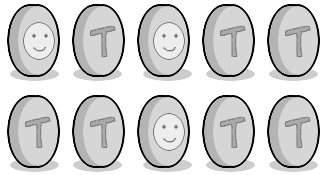
\includegraphics[width=10cm]{images/6-3-coins.png}
        \end{center}

        \vspace{1cm}
        
        $n$, the amount of trial repeats:
        
        \vspace{1cm}
        
        $k$, the amount of successes (heads):
        
        \vspace{1cm}
        
        $p$, the probability of success:

        ~\\~\\
        Use the formula of $ C(n, k) \cdot p^{k} \cdot (1 - p)^{n-k} $
        to find the probability.
    \end{questionNOGRADE}

    \newpage

        
        % -------------------------------------------------------------%
        % - QUESTION --------------------------------------------------%
    \stepcounter{question}
    \begin{questionNOGRADE}{\thequestion}
        % Exercise 2
        What is the probability that in seven rolls of a six-sided die,
        the result of 1 appears \textit{at least} five times?

        \begin{center}
            
\includegraphics[width=12cm]{images/6-3-dice.png}
        \end{center}

        \begin{hint}{Hint}
            For this one, we will need to use the \textbf{rule of sums}
            to combine several outcomes: Getting 5 1's, 6 1's, OR 7 1's.
        \end{hint}

        \large
        \begin{center}
            \begin{tabular}{ | c | p{4cm} | c | c | c | }
                \hline
                & & repeats $n$ & successes $k$ & probability $p$
                \\ \hline
                A &
                Getting five 1's
                    & \solution{ $ 7 $ }{ 7 }
                    & \solution{ $ 5 $ }{ 5 }
                    & \solution{ 1/6 }{ 1/6 }
                \\ \hline
                B &
                Getting six 1's
                    & \solution{ $ 7 $ }{ 7 }
                    & \solution{ $ 6 $ }{}
                    & \solution{ 1/6 }{}
                \\ \hline
                C &
                Getting seven 1's
                    & \solution{ $ 7 $ }{ 7 }
                    & \solution{ $ 7 $ }{}
                    & \solution{ 1/6 }{}
                \\ \hline
            \end{tabular}
        \end{center}
        \normalsize

        Now, using the formula $ C(n, k) \cdot p^{k} \cdot (1 - p)^{n-k} $
        three different times for case (A), (B), and (C).

        ~\\ (A) \tab $ C(n, k) \cdot p^{k} \cdot (1 - p)^{n-k} $ =
        ~\\ \vspace{1cm}
        
        ~\\ (B) \tab $ C(n, k) \cdot p^{k} \cdot (1 - p)^{n-k} $ =
        ~\\ \vspace{1cm}
        
        ~\\ (C) \tab $ C(n, k) \cdot p^{k} \cdot (1 - p)^{n-k} $ =
        ~\\ \vspace{1cm}

        To find the probability of getting at least five 1's in seven rolls,
        add (A), (B), and (C) together. (Just write out the formula; don't solve.)

        ~\\
        $Prob($ at least five 1's $) = $
    \end{questionNOGRADE}

        \notonkey{ \newpage }{ \hrulefill }
        
        % -------------------------------------------------------------%
        % - QUESTION --------------------------------------------------%
        % -------------------------------------------------------------%
        \stepcounter{question}
        \begin{question}{\thequestion}{3}
            % Exercise 5
            What is the probability of getting exactly one 6 on 10 tosses
            of a fair six-sided die?            
        \end{question}


}{
% KEY ------------------------------------ %

    \begin{enumerate}
        \item
            \begin{itemize}
                \item   $n = 10$
                \item   $k = 3$
                \item   $p = 1/2$
                \item   $ C(10, 3) \cdot (1/2)^{3} \cdot (1/2)^{7} = \frac{15}{128}$
            \end{itemize}

        \item
            \begin{itemize}
                \item   
                    \begin{tabular}{ | c | p{4cm} | c | c | c | }
                        \hline
                        & & repeats $n$ & successes $k$ & probability $p$
                        \\ \hline
                        A & Getting five 1's & 7 & 5 & 1/6
                        \\ \hline
                        B & Getting six 1's & 7 & 6 & 1/6
                        \\ \hline
                        C & Getting seven 1's & 7 & 7 & 1/6
                        \\ \hline
                    \end{tabular}
                
                \item[A.]   $ C(n, k) \cdot p^{k} \cdot (1 - p)^{n-k} $ = $C(7,5) \cdot (1/6)^{5} \cdot (5/6)^{2}$
                \item[B.]   $ C(n, k) \cdot p^{k} \cdot (1 - p)^{n-k} $ = $C(7,6) \cdot (1/6)^{6} \cdot (5/6)^{1}$
                \item[C.]   $ C(n, k) \cdot p^{k} \cdot (1 - p)^{n-k} $ = $C(7,7) \cdot (1/6)^{7} \cdot (5/6)^{0}$
                \item   $Prob($ at least five 1's $) = $
                        $C(7,5) \cdot (1/6)^{5} \cdot (5/6)^{2} +
                        C(7,6) \cdot (1/6)^{6} \cdot (5/6)^{1} +
                        C(7,7) \cdot (1/6)^{7} \cdot (5/6)^{0}$
            \end{itemize}
        \item   $n = 10$, $k = 1$, $p = (1/6)$ \\
                $C(10,1) \cdot (1/6)^{1} \cdot (5/6)^{9} \approx 0.323 $
    \end{enumerate}

}



\end{document}

